
%%%%%%%%%%%%%%%%%%%%%%%%%%%%%%%%%%%%%%%%%%%%%%%%%%%%%%%%%%%%%%%%%%%%%%%%%%%%
\chapter{ΕΦΑΡΜΟΓΕΣ ΧΡΟΝΟΣΕΙΡΩΝ ΜΕ ΤΙΣ ΜΕΘΟΔΟΥΣ ΕΞΟΜΑΛΥΝΣΗΣ ΚΑΙ ΔΙΑΣΠΑΣΗΣ ΧΡΟΝΟΣΕΙΡΩΝ }
%%%%%%%%%%%%%%%%%%%%%%%%%%%%%%%%%%%%%%%%%%%%%%%%%%%%%%%%%%%%%%%%%%%%%%%%%%%%
%%%%%%%%%%%%%%%%%%%%%%%%%%%%%%%%%%%%%%%%%%%%%%%%%%
\section{ΠΡΟΒΛΕΨΗ ΤΙΜΩΝ ΧΡΟΝΟΣΕΙΡΑΣ ΜΕ ΤΗ ΜΕΘΟΔΟ ΔΙΑΣΠΑΣΗΣ ΧΡΟΝΟΣΕΙΡΩΝ}
%%%%%%%%%%%%%%%%%%%%%%%%%%%%%%%%%%%%%%%%%%%%%%%%%%
%%%%%%%%%%%%%%%%%%%%%%%%%%%%%%%%%%%%%%%%%%%%%%%%%%
\textbf{Παράδειγμα 3.1}\\\\
Στον πίνακα \ref{tab_1} που ακολουθεί παρουσιάζεται
η ανάλυση της εποχικότητας, της μακροχρόνιας τάσης και των κυκλικών διακυμάνσεων, αναφορικά με τις πωλήσεις των αυτοκινήτων στην Ελλάδα. Έπειτα από την ολοκλήρωση των αναλύσεων αυτών, παραθέτουμε τις προβλέψεις για τις πωλήσεις των αυτοκινήτων στην Ελλάδα, που αφορούν τα τρίμηνα του 2005
και του 2006.
\begin{table} [h]
  \caption{Δεδομένα, εποχικοί δείκτες και τιμές απαλλαγμένες από εποχικότητα.} 
  \label{tab_1}
  \begin{center}
    \begin{tabular}{|c|c|c|c|c|c|c|c|}
      \hline
           &         &              &          &         
           &         &              &          \\
           &         &              &          &
           & Κεντρικός  &     & Τιμές \\
           &  &  &  & Κινητός & Κινητός  & Εποχικοί &Απαλλαγμένες
            \\
      Έτος & Τρίμηνο & Περίοδος  & Πωλήσεις  & Μέσος  & Μέσος  & Δείκτες  & Εποχικότητας  \\
   &   & t & $Y_t $ & MA & $ CA_t$ & $ S_t$ & $SAY_t $ \\
      \hline \hline
      2000 &  1o  &  1  &  83.754  &  -  &  -  &   -  &  76.371,48\\
           &  2o  &  2  &  83.121  &  72.555,50  &  -  &  -  &  72.576,98\\
           & 3ο & 3  &  68.976 & 70.930,25  & 71.742,88  & 0,9614 & 70.538,78 \\
           & 4ο & 4 & 54.371 & 70.588,75 & 70.759,50  & 0,7684 & 69.687,79 \\
           
        2001   & 1ο & 5  & 77.253  &70.700,75  &70.644,75  & 1,0935 &70.443,51\\
        & 2ο & 6 & 81.755 &70.053,50 &70.377,13  & 1,1617 &71.384,26\\
        & 3ο & 7  &69.424  & 68.683,25 & 69.368,38 & 1,0008 & 70.996,93\\
        & 4ο &8  & 51.782 & 67.187,25 &67.935,25 & 0,7622 & 66.369,44\\
     2002   & 1o & 9 & 71.772 & 67.224,50 & 67.205,88  & 1,0679 & 65.445,64 \\
     & 2o  & 10 & 75.771 & 67.122,25 & 67.173,38 & 1,1280 & 66.159,34\\
     & 3o & 11 & 69.573 & 66.717,50 & 66.919,88 & 1,0396 & 71.149,30\\
     & 4o & 12 & 51.373 & 65.541,50 &66.129,50 &0,7769  &65.845,22\\
   2003  & 1o & 13 &70.153  & 63.125,50 & 64.333,50 & 1,0905  &63.969,34\\
     & 2o & 14 &71.067 & 64.323,25 & 63.724,38 & 1,1152 & 62.052,05\\
     & 3o & 15 & 59.909  & 67.129,25 & 65.726,25  & 0,9115 &61.266,35\\
      & 4o & 16 & 56.164 & 70.704,50 & 68.916,88  & 0,8150 & 71.985,89\\
      2004& 1o &  17& 81.377 & 72.444,25 & 71.574,38 & 1,1370 &74.204,00\\
      & 2o & 18 & 85.368 & 72.422,75  & 72.433,50 & 1,1786 &74.538,95\\
      & 3o &19  & 66.868 & - & - & - &68.383,02\\
      & 4o & 20 & 56.078 & - & - & - &71.875,66\\
     
      \hline
    \end{tabular}
  \end{center}
\end{table}

\begin{table} [h]
  \caption{Προσαρμοσμένοι Εποχικοί Δείκτες.} 
  \label{tab_2}
  \begin{center}
    \begin{tabular}{|c|c c c c|c|}
      \hline
      &  &  &  &  &\\
      &  &  Τρίμηνο &  &  & \\
   Έτος   & 1ο & 2ο & 3ο  & 4ο  & Άθροισμα \\
   \hline \hline
   2000&   &  & 0,961 &0,768  &  \\
   2001  &1,094  & 1,162 & 1,001 &0,762 &  \\
   2002& 1,068 & 1,128 & 1,040 & 0,777 &  \\
    2003& 1,090 & 1,115 & 0,911 & 0,815 &  \\  
    2004& 1,137 & 1,179 &  &  &  \\
    \hline
    Άθροισμα & 4,389 & 4,583 &3,913  & 3,122 &  \\
    Μέσοι& 1,097 & 1,146 & 0,978 & 0,781 & 4,0020 \\
    Προσαρμοσμένοι Δείκτες& 1,097 &1,145 & 0,978 & 0,780 & 4,0000 \\
      \hline
    \end{tabular}
  \end{center}
\end{table}

\begin{figure} [ht]
  \centering
  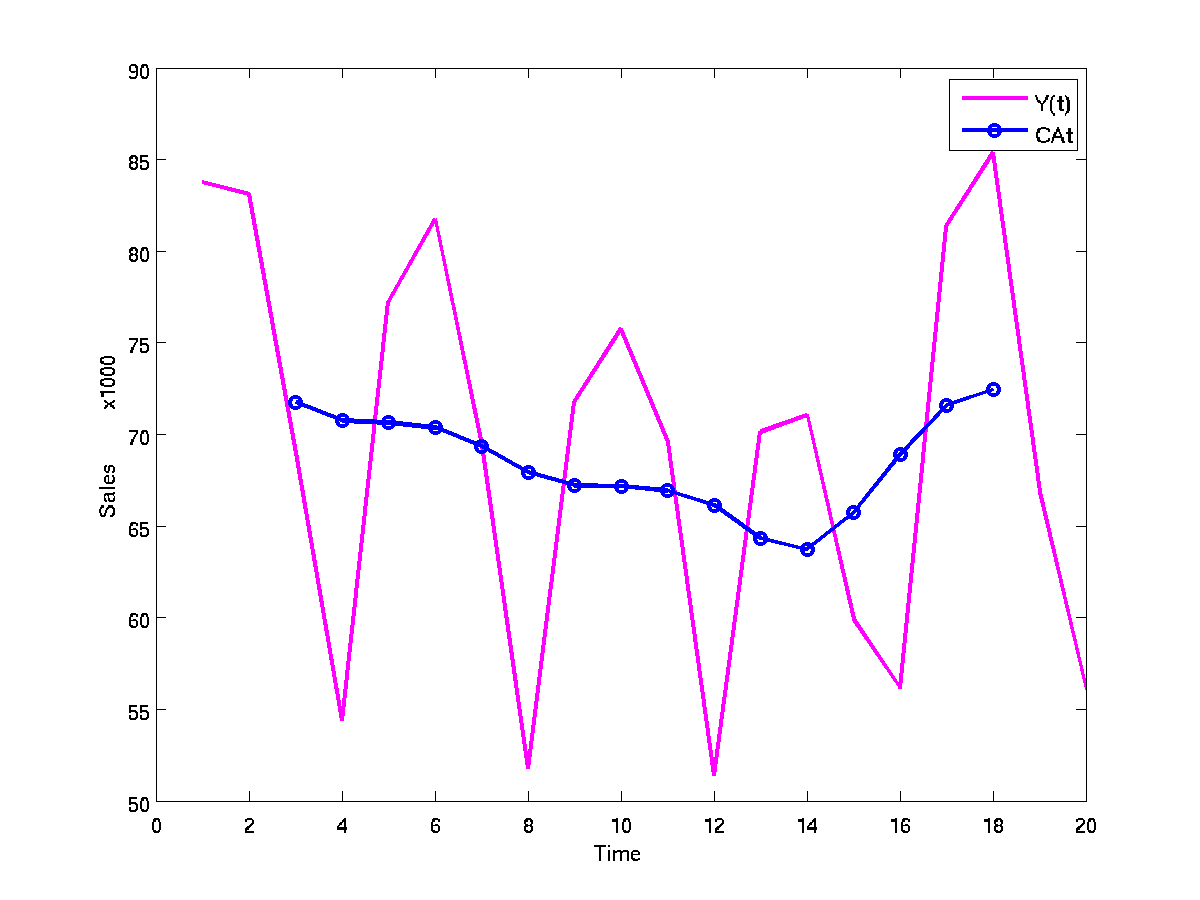
\includegraphics[totalheight=3.2in,angle=0]{graff2.png}
  \caption{Εξομάλυνση των δεδομένων του παραδείγματος 3.1 με κεντρικό κινητό μέσο.}
%  \label{fig:figure5}
\end{figure}
 
\begin{figure} [ht]
  \centering
  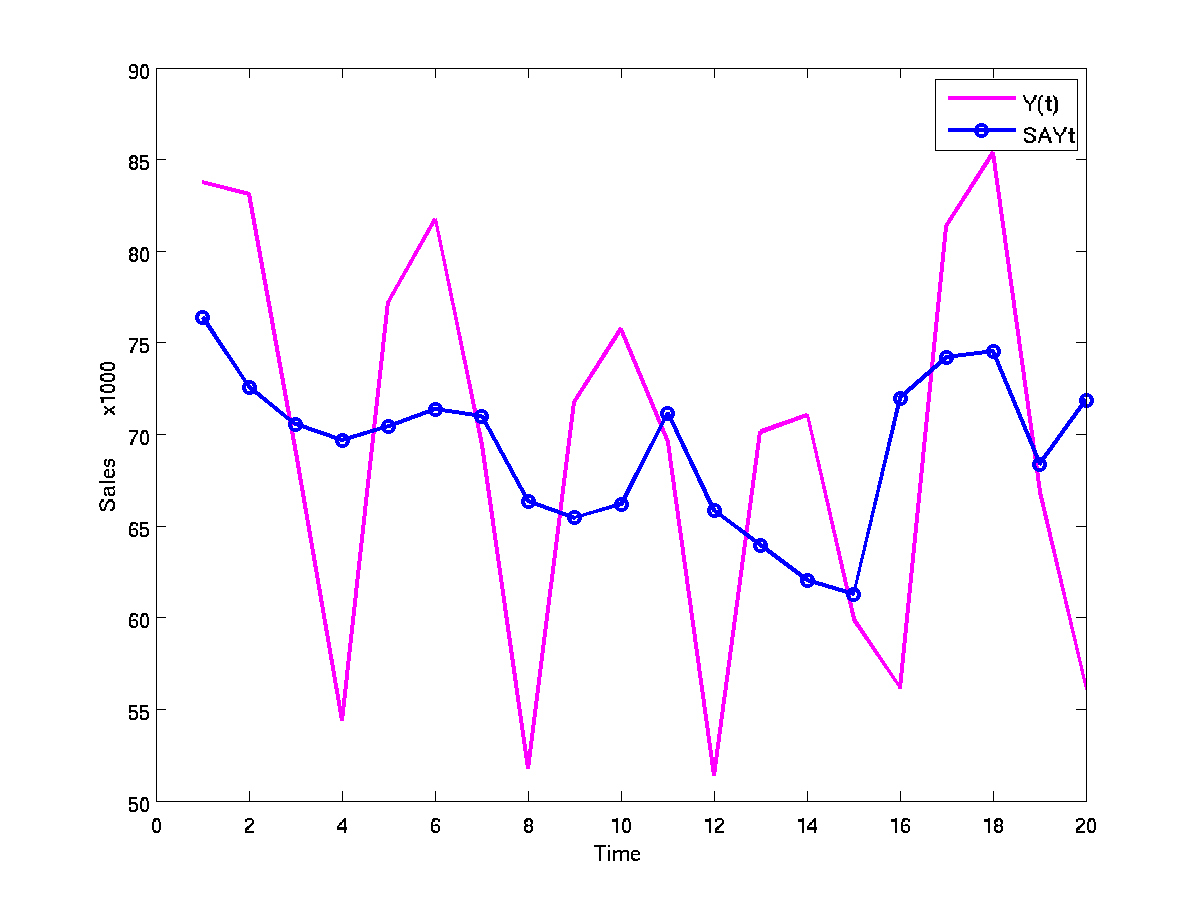
\includegraphics[totalheight=3.2in,angle=0]{graff3.png}
  \caption{Πραγματικές και απαλλαγμένες από εποχικότητα τιμές της χρονοσειράς του παραδείγματος 3.1.}
\end{figure}

\begin{table} [h]
  \caption{Προσδιορισμός Μακοχρόνιας Τάσης για τις πωλήσεις αυτοκινήτων.} 
  \label{tab_3}
  \begin{center}
    \begin{tabular}{|c|c|c|c|c|c|c|c|}
      \hline
           &   &    &    &         
           &   &    &      \\
           &    &     &    & Τιμές
           &  &     &  \\
           &  &  &  &Απαλλαγμένες &  &  &\\
       Έτος &Τρίμηνο  &Περίοδος  &Πωλήσεις  &Εποχικότητας  &  &  & Τάση \\
       & & t  & $Y_t$  & $ SAY_t$  & $t^2$  & $t*SAY_t$  &   \\
      \hline \hline
      2000 &  1o  &  1  &  83.754  &  76.371,48  &  1  & 76.371,48  &  70.551,67\\
           &  2o  &  2  &  83.121  &  72.576,98  &  4  & 145.153,96  &  70.415,93\\
           & 3ο & 3  &  68.976 & 70.538,78  & 9  & 211.616,34 & 70.280,20 \\
           & 4ο & 4 & 54.371 & 69.687,79 & 16  & 278.751,16 & 70.144,46 \\
           
        2001   & 1ο & 5  & 77.253  & 70.443,51  &  25 & 352.217,55 &  70.008,73\\
        & 2ο & 6 & 81.755 & 71.384,26 & 36  & 428.305,56 & 69.873,00\\
        & 3ο & 7  &69.424  & 70.996,93 & 49 & 496.978,51 & 69.737,26\\
        & 4ο &8  & 51.782 & 66.369,44 & 64 & 530.955,52 & 69.601,53\\
     2002   & 1o & 9 & 71.772 & 65.445,64 & 81 & 589.010,76 & 69.465,80 \\
     & 2o  & 10 & 75.771 & 66.159,34 & 100 & 661.593,40 & 69.330,06\\
     & 3o & 11 & 69.573 & 71.149,30 & 121 & 782.642,30 & 69.194,33\\
     & 4o & 12 & 51.373 & 65.845,22 &  144 & 790.142,64 &69.058,60\\
   2003  & 1o & 13 &70.153  & 63.969,34 & 169 & 831.601,42  &68.922,86\\
     & 2o & 14 &71.067 & 62.052,05 & 196 & 868.728,70 & 68.787,13\\
     & 3o & 15 & 59.909  & 61.266,35 & 225  & 918.995,25 &68.651,40\\
      & 4o & 16 & 56.164 & 71.985,89 & 256 & 1.151.774,24 & 68.515,66\\
      2004& 1o &  17& 81.377 & 74.204,00 & 289 & 1.261.468,00 & 68.379,93\\
      & 2o & 18 & 85.368 & 74.538,95  & 324 & 1.341.701,10 &68.244,20\\
      & 3o &19  & 66.868 & 68.383,02 & 361 & 1.299.277,38 &68.108,46\\
      & 4o & 20 & 56.078 & 71.875,66 & 400 & 1.437.513,20 &67.972,73\\    
      \hline
    \end{tabular}
  \end{center}
\end{table}
%%%%%%%%%%% mou ta emfanizei pio panw auta ta logia
Παρακάτω δίνεται η γραφική παράσταση των απαλλαγμένων από εποχικότητα τιμών της χρονοσειράς καθώς επίσης και η γραφική παράσταση της εκτιμηθείσας γραμμικής τάσης των τιμών της
χρονοσειράς.

\begin{figure} [ht]
  \centering
  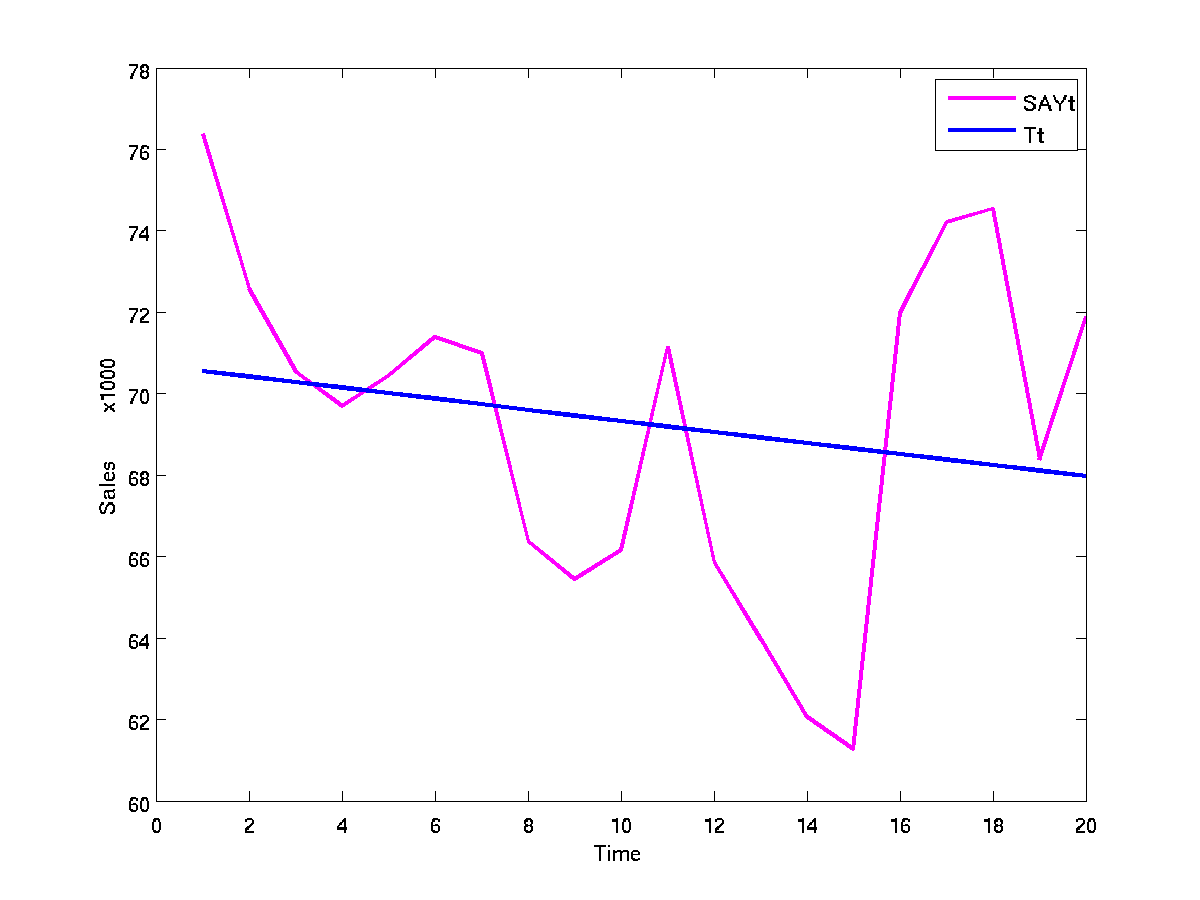
\includegraphics[totalheight=4in,angle=0]{graff4.png}
  \caption{Τιμές χρονοσειράς απαλλαγμένες από εποχικότητα και οι αντίστοιχες τιμές της τάσης του παραδείγματος 3.1.}
\end{figure}


\begin{table} [h]
  \caption{Προσδιορισμός Κυκλικών Διακυμάνσεων των πωλήσεων των αυτοκινήτων.} 
  \label{tab_4}
  \begin{center}
    \begin{tabular}{|c|c|c|c|c|c|c|c|}
      \hline
           &   &   &   &
           &   &  &Σταθμισμ.      \\
           &   &   &
           & Τιμές   &     &Τιμές    & κεντρικός   \\
          &   &   & 
           &Απαλλαγμένες  &  &Απαλλαγμένες  &κιν. Μέσος  \\
          Έτος  &Τρίμηνο  & Περίοδος & Πωλήσεις
            &Εποχικότητας  & Τάση  & από Τάση   &Όρος  \\
        &  & t  &$ Y_t$  &$ SAY_t$  &  & $ TAY_t$ & $ WA_t$ \\
      \hline \hline
      2000 &  1o  &  1  &  83.754  &  76.371,48  &  70.551,67  & 1,082  &  -\\
           &  2o  &  2  &  83.121  &  72.576,98  &  70.415,93  & 1,031  &  1,037\\
           & 3ο & 3  &  68.976 & 70.538,78  & 70.280,20  & 1,004 & 1,008 \\
           & 4ο & 4 & 54.371 & 69.687,79 & 70.144,46  & 0,993 & 0,999 \\
           
        2001   & 1ο & 5  & 77.253  & 70.443,51  &  70.008,73 & 1,006 &  1,007\\
        & 2ο & 6 & 81.755 & 71.384,26 & 69.873,00  & 1,022 & 1,017\\
        & 3ο & 7  &69.424  & 70.996,93 & 69.737,26 & 1,018 &1,003 \\
        & 4ο &8  & 51.782 & 66.369,44 & 69.601,53 & 0,954 & 0,967\\
     2002   & 1o & 9 & 71.772 & 65.445,64 & 69.465,80 & 0,942 & 0,948 \\
     & 2o  & 10 & 75.771 & 66.159,34 & 69.330,06 & 0,954 & 0,970\\
     & 3o & 11 & 69.573 & 71.149,30 & 69.194,33 & 1,028 & 0,991\\
     & 4o & 12 & 51.373 & 65.845,22 &  69.058,60 & 0,953 &0,966\\
   2003  & 1o & 13 &70.153  & 63.969,34 & 68.922,86 & 0,928  &0,928\\
     & 2o & 14 &71.067 & 62.052,05 & 68.787,13 & 0,902& 0,906\\
     & 3o & 15 & 59.909  & 61.266,35 &68.651,40  & 0,892 &0,934\\
      & 4o & 16 & 56.164 & 71.985,89 & 68.515,66 & 1,051 & 1,020\\
      2004& 1o &  17& 81.377 & 74.204,00 & 68.379,93 & 1,085 & 1,078\\
      & 2o & 18 & 85.368 & 74.538,95  & 68.244,20 &1,092 &1,068\\
      & 3o &19  & 66.868 & 68.383,02 & 68.108,46 & 1,004 &1,039\\
      & 4o & 20 & 56.078 & 71.875,66 & 67.972,73 & 1,057 &-\\
     
      \hline
    \end{tabular}
  \end{center}
\end{table}
%%%%%%%%%%%%%%mou ta emfanizei pio panw ayta ta logia
Οι απαλλαγμένες από τάση και εποχικότητα τιμές του παραπάνω παραδείγματος, περιέχουν μόνο την
κυκλικότητα και τη μη κανονικότητα. Παρακάτω δίνεται η γραφική παράσταση των απαλλαγμένων από τάση και εποχικότητα τιμών της χρονοσειράς (TAYt) και η γραφική παράσταση των τιμών του σταθμικού κεντρικού κινητού μέσου (WAt).
\begin{figure} [ht]
  \centering
  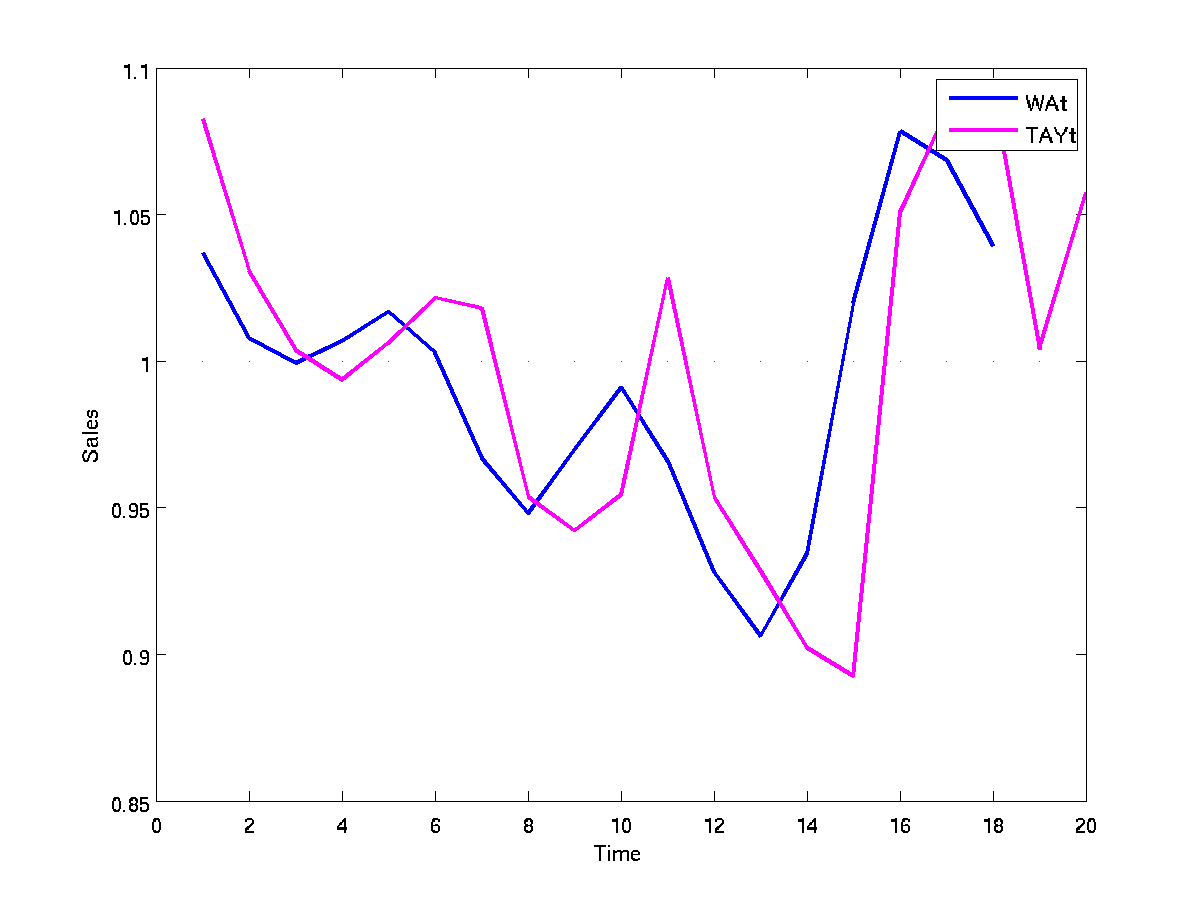
\includegraphics[totalheight=3.2in,angle=0]{graff6.png}
  \caption{Τιμές χρονοσειράς απαλλαγμένες από τάση και από εποχικότητα του παραδείγματος 3.1 και τιμές του σταθμικού κεντρικού κινητού μέσου.}
\end{figure}

\begin{table} [h]
  \caption{Προβλέψεις για τα επόμενα δύο έτη.} 
  \label{tab_5}
  \begin{center}
    \begin{tabular}{|c |c | c| c|}
      \hline 
       &  &  &  \\
       Έτος &Τρίμηνο   &Περίοδος   &Προβλέψεις  \\
       &   & t  & $\widehat{Y}_t$  \\    
       \hline \hline
       2005 & 1o & 21 & 74.395 \\
            & 2o & 22 & 77.537 \\
            & 3o & 23 & 66.069 \\
            & 4o & 24 & 52.609 \\
       2006 & 1o & 25 & 73.799 \\
            & 2o & 26 & 76.915 \\
            & 3o & 27 & 65.538 \\
            & 4o & 28 & 52.186 \\     
      \hline
    \end{tabular}
  \end{center}
\end{table}

\begin{figure} [ht]
  \centering
  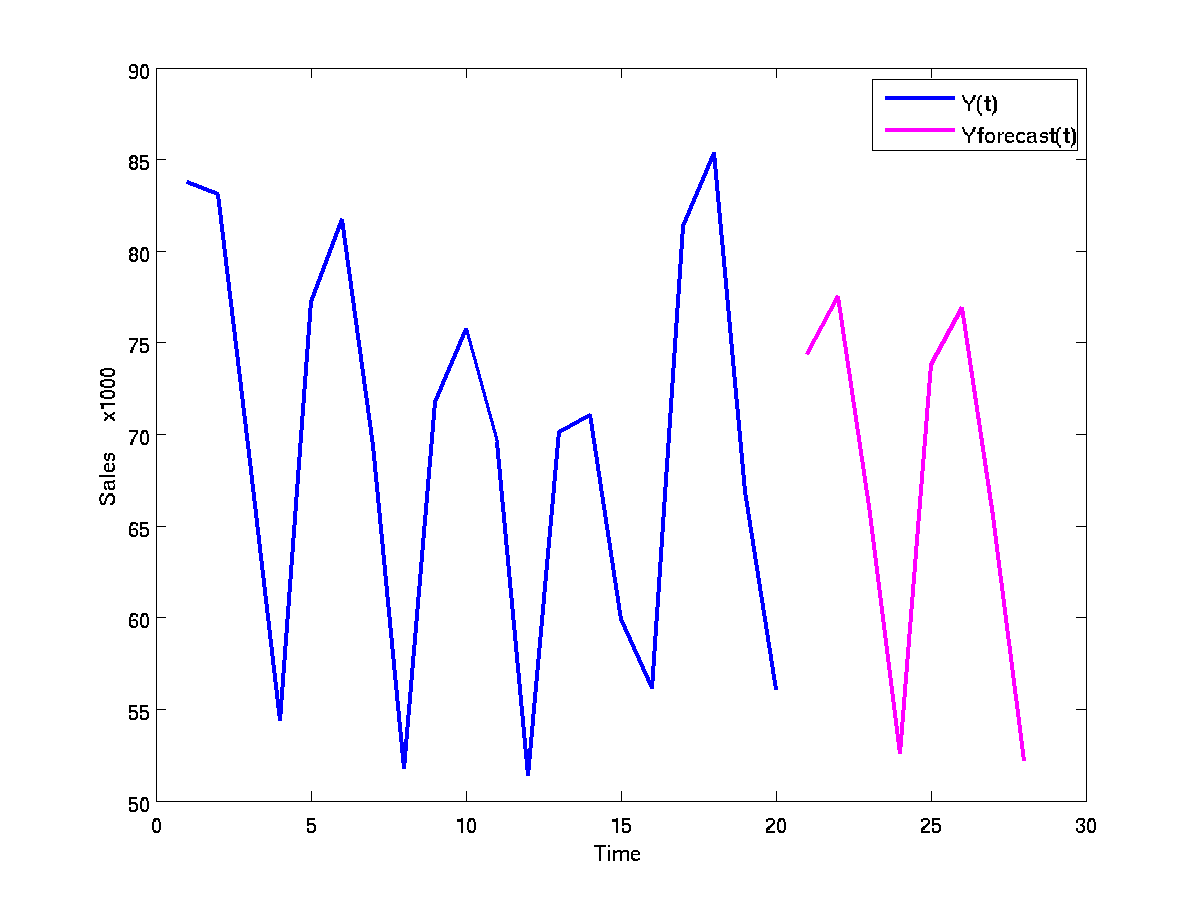
\includegraphics[totalheight=3.2in,angle=0]{graff7.png}
  \caption{Πραγματικές τιμές της χρονοσειράς και οι προβλεπόμενες τιμές για το έκτο και έβδομο έτος.}
\end{figure}

\begin{table} [h]
  \caption{Προσδιορισμός Κυκλικών Διακυμάνσεων των πωλήσεων των αυτοκινήτων.} 
  \label{tab_4}
  \begin{center}
    \begin{tabular}{|c|c|c|c|c|c|c|c|c|}
      \hline
           &   &   &   &
           &   &  &   &     \\
           Έτος & Τρίμηνο  & Πείοδος  & Πωλήσεις  & $ A_t$
           & $T_t$   & $ S_t$  & $ \widehat{Y}_t$  & $ e_t$ \\
      \hline \hline
      2000 &  1o  &  1  &  83.754  &    &     & 1,15 &  & \\
           &  2o  &  2  &  83.121  &    &   & 1,15  &  & \\
           & 3ο & 3  &  68.976 &   &  & 0,95 &  &  \\
           & 4ο & 4 & 54.371 & 72.555,50 & 0,00  & 0,75 &  &  \\
           
        2001   & 1ο & 5  & 77.253  & 69.121,08  & -34,34 & 1,14 & 83.754,00 & -6.501,00\\
        & 2ο & 6 & 81.755 & 70.474,95 & -20,46  & 1,15 & 79.147,11 &2.607,89 \\
        & 3ο & 7  &69.424  & 72.023,13 & -4,78 & 0,95 &66.978,64 & 2.445,36 \\
        & 4ο &8  & 51.782 & 70.239,02 & -22,57 & 0,75 & 53.968,48 & -2.186,48\\
     2002   & 1o & 9 & 71.772 & 65.700,57 & -67,73 & 1,13 & 80.233,57 & -8.461,57 \\
     & 2o  & 10 & 75.771 & 65.780,78 & -66,25 & 1,15 & 75.491,97 & 279,03\\
     & 3o & 11 & 69.573 & 70.072,20 & -22,67 & 0,97 & 62.749,69 & 6.823,31\\
     & 4o & 12 & 51.373 & 69.354,86 & -29,62 & 0,74 &52.222,22 & -849,22\\
   2003  & 1o & 13 &70.153  & 65.020,45 & -72,67 & 1,11  &78.106,10 &-7.953,10\\
     & 2o & 14 &71.067 & 63.002,24 & -92,12 & 1,14& 74.738,23 & -3.671,23\\
     & 3o & 15 & 59.909  & 62.327,53 & -97,95  & 0,97 & 60.832,78 & -923,78\\
      & 4o & 16 & 56.164 & 70.316,76 & -17,08 & 0,76 & 46.297,77 & 9.866,23\\
      2004& 1o &  17& 81.377 & 72.078,03 & 0,71 & 1,12 & 78.135,81 &3.241,19 \\
      & 2o & 18 & 85.368 & 73.649,64  & 16,42 & 1,15 & 82.422,38 &2.945,62 \\
      & 3o &19  & 66.868 & 70.993,35 & -10,31 & 0,96 &71.097,92 &-4.229,92 \\
      & 4o & 20 & 56.078 & 72.609,38 & 5,95 & 0,76 &54.047,41 & 2.030,59\\
      2005 & 1o  & 21 &  &  &  &  &81.115  &  \\
      & 2o & 22 &  &  &  &  & 83.404  &  \\
      & 3o & 23 &  &  &  &  & 69.558 &  \\
      & 4o & 24 &  &  &  &  & 55.556  &  \\
      2006& 1o & 25 &  &  &  &  & 81.142 &  \\
      & 2o &26  &  &  &  &  & 83.431 &  \\
      & 3o & 27 &  &  &  &  &69.581  &  \\
      & 4o & 28 &  &  &  &  & 55.574 &  \\
     
      \hline
    \end{tabular}
  \end{center}
\end{table}
%\begin{center}
%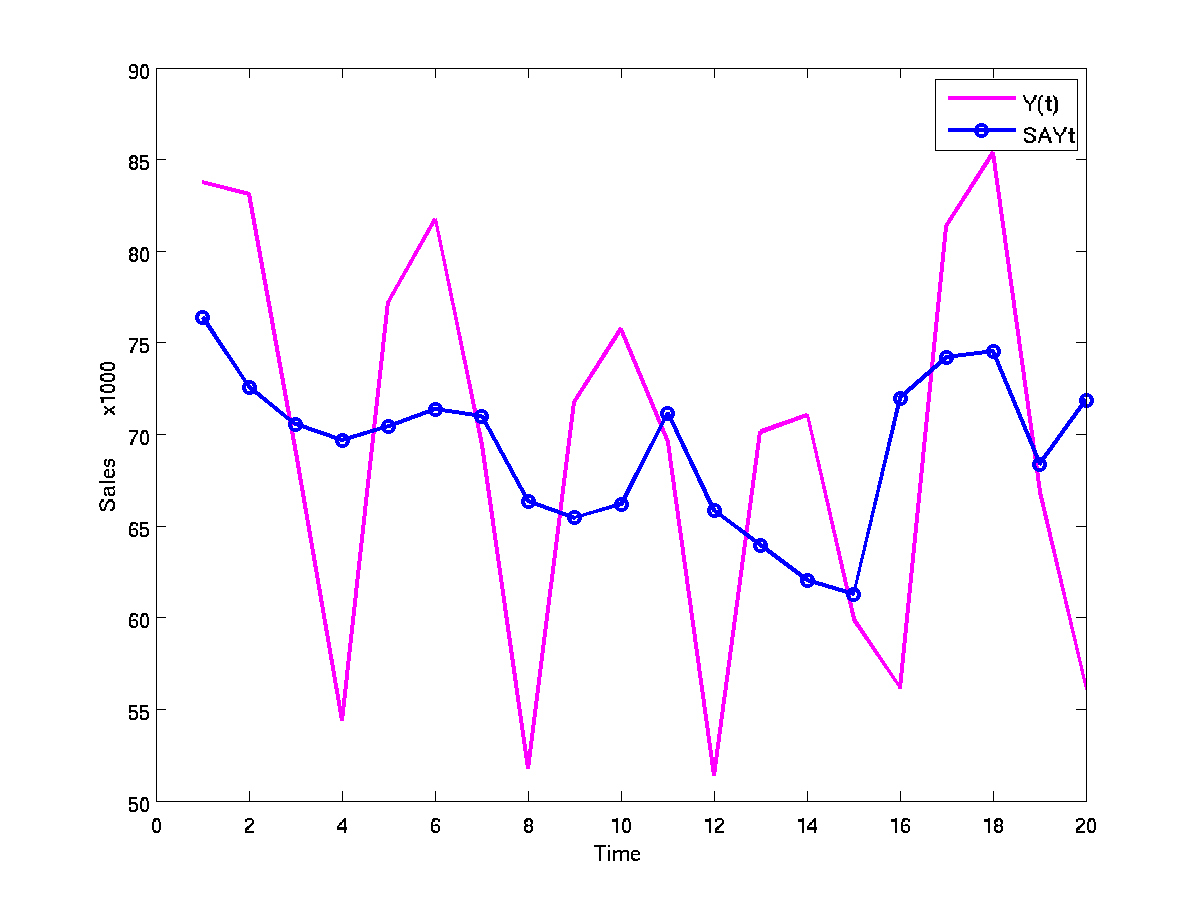
\includegraphics[scale=0.7]{graff3.png}\\   
%\textbf{Σχήμα 3.1: Γράφημα χρονοσειράς}
%\end{center} 
%%%%%%%%%%%%%%%%%%%%%%%%%%%%%%%%%%%%%%%%%%%%%%%%%%%%%%%%%%%%%%%%%%%%%%%%%%%%%%%%%%%%%%%%%%%%%%%%%%%%
%\subsection{Όνομα πρώτης υποενότητας}
%%%%%%%%%%%%%%%%%%%%%%%%%%%%%%%%%%%%%%%%%%%%%%%%%%%%%%%%%%%%%%%%%%%%%%%%%%%%%%%%%%%%%%%%%%%%%%%%%%%%
%%%%%%%%%%%%%%%%%%%%%%%%%%%%%%%%%%%%%%%%%%%%%%%%%%%%%%%%%%%
%\section{ΒΡΑΧΥΠΡΟΘΕΣΜΕΣ ΠΡΟΒΛΕΨΕΙΣ ΧΡΗΣΙΜΟΠΟΙΩΝΤΑΣ ΤΗ ΜΕΘΟΔΟ WINTERS}
%%%%%%%%%%%%%%%%%%%%%%%%%%%%%%%%%%%%%%%%%%%%%%%%%%%%%%%%%%%





%%%%%%%%%%%%%%% File ends here %%%%%%%%%%%%%%%%%%%%%%%%%%%%%%%%
\endinput
%%% Local Variables: 
%%% mode: latex
%%% TeX-master: "ptyxiakn"
%%% End: 
